% answers.tex —— 2015 年·广东卷·文科 · 参考答案与详细解析片段
% 由 tools/generate_projects.py 依来源总账自 2015/2015_数学真题_广东文_试题.md + 2015/2015_数学真题_广东文_解析正文.md + 2015/2015_数学真题_广东文_答案要点.md 生成，勿手改（改源 MD 后重跑）

\begin{answer}
\gksolhead{1}{}

\textbf{题目}：

若集合 \(M=\{-1,1\}\)，\(N=\{-2,1,0\}\)，则 \(M\cap N=\)（　）

(A) \(\{0,-1\}\)　(B) \(\{1\}\)　(C) \(\{0\}\)　(D) \(\{-1,1\}\)

\Needspace{4\baselineskip}
\textbf{解析}

\Needspace{5\baselineskip}
由 \(M=\{-1,1\}\)，\(N=\{-2,1,0\}\)，交集由同时属于两个集合的元素组成。逐一检验 \(M\) 中的元素：\(-1\notin N\)（\(N\) 的元素为 \(-2\)，\(1\)，\(0\)），而 \(1\in N\)。故

\nopagebreak[4]
\[
M\cap N=\{1\}.
\]

故选 (B)。

（验证：① 反向核对：\(\{1\}\subset M\) 且 \(\{1\}\subset N\)；\(0\in N\) 但 \(0\notin M\)，\(-2\in N\) 但 \(-2\notin M\)，故再无其他公共元素。② 计数校验：\(\operatorname{card}\,(M\cap N)=1\)，且 \(\operatorname{card}\,(M\cup N)=2+3-1=4\)，与 \(M\cup N=\{-2,-1,0,1\}\) 的四个元素一致。）

\gkanswer{答案：B（\(\{1\}\)）}

\end{answer}
\begin{answer}
\gksolhead{2}{}

\textbf{题目}：

已知 \(\mathrm{i}\) 是虚数单位，则复数 \((1+\mathrm{i})^2=\)（　）

(A) \(2\mathrm{i}\)　(B) \(-2\mathrm{i}\)　(C) \(2\)　(D) \(-2\)

\Needspace{4\baselineskip}
\textbf{解析}

\Needspace{5\baselineskip}
按复数乘法展开，并利用 \(\mathrm{i}^2=-1\)：

\nopagebreak[4]
\[
(1+\mathrm{i})^2=1+2\mathrm{i}+\mathrm{i}^2=1+2\mathrm{i}-1=2\mathrm{i}.
\]

故选 (A)。

（验证：① 模与辐角路径：\(|1+\mathrm{i}|=\sqrt{2}\)，\(\arg(1+\mathrm{i})=\dfrac{\pi}{4}\)，平方后模为 \(2\)、辐角为 \(\dfrac{\pi}{2}\)，即 \(2\mathrm{i}\)。② 逐项相乘：\((1+\mathrm{i})(1+\mathrm{i})=1+\mathrm{i}+\mathrm{i}+\mathrm{i}^2=2\mathrm{i}\)。）

\gkanswer{答案：A（\(2\mathrm{i}\)）}

\end{answer}
\begin{answer}
\gksolhead{3}{}

\textbf{题目}：

下列函数中，既不是奇函数，也不是偶函数的是（　）

(A) \(y=x+\sin 2x\)　(B) \(y=x^2-\cos x\)

(C) \(y=2^x+\dfrac{1}{2^x}\)　(D) \(y=x^2+\sin x\)

\Needspace{4\baselineskip}
\textbf{解析}

四个函数的定义域均为 \(\mathbf{R}\)。记所给函数为 \(f(x)\)，分别计算 \(f(-x)\)。

(A) \(f(-x)=-x+\sin(-2x)=-x-\sin 2x=-f(x)\)，为奇函数。

(B) \(f(-x)=(-x)^2-\cos(-x)=x^2-\cos x=f(x)\)，为偶函数。

(C) \(f(-x)=2^{-x}+\dfrac{1}{2^{-x}}=2^{-x}+2^{x}=f(x)\)，为偶函数。

(D) \(f(-x)=x^2+\sin(-x)=x^2-\sin x\)。若 \(f(-x)=f(x)\)，则需 \(-2\sin x=0\) 对一切 \(x\) 成立，不成立；若 \(f(-x)=-f(x)\)，则需 \(2x^2=0\) 对一切 \(x\) 成立，同样不成立。故 (D) 既不是奇函数也不是偶函数。

故选 (D)。

（验证：① 取 \(x=\dfrac{\pi}{2}\) 代入 (D)：\(f\left(\dfrac{\pi}{2}\right)=\dfrac{\pi^2}{4}+1\)，\(f\left(-\dfrac{\pi}{2}\right)=\dfrac{\pi^2}{4}-1\)，后者既不等于前者，也不等于前者的相反数。② 对 (A)(B)(C)，\(f(-x)\) 与 \(f(x)\) 或 \(-f(x)\) 的恒等式已逐项算出；(D) 的 \(f(-x)-f(x)=-2\sin x\) 与 \(f(-x)+f(x)=2x^2\) 均不恒为零。）

\gkanswer{答案：D（\(y=x^2+\sin x\)）}

\end{answer}
\begin{answer}
\gksolhead{4}{}

\textbf{题目}：

\Needspace{5\baselineskip}
若变量 \(x\)，\(y\) 满足约束条件

\nopagebreak[4]
\[
\begin{cases}
x+2y\leqslant 2,\\
x+y\geqslant 0,\\
x\leqslant 4,
\end{cases}
\]

则 \(z=2x+3y\) 的最大值为（　）

(A) \(2\)　(B) \(5\)　(C) \(8\)　(D) \(10\)

\Needspace{4\baselineskip}
\textbf{解析}

可行域由三条边界直线 \(x+2y=2\)，\(x+y=0\)，\(x=4\) 围成。由 \(y\geqslant -x\) 与 \(y\leqslant 1-\dfrac{x}{2}\) 得 \(-x\leqslant 1-\dfrac{x}{2}\)，即 \(x\geqslant -2\)；结合 \(x\leqslant 4\) 知可行域有界。

三组边界直线的交点：

\begin{itemize}
\item \(x+2y=2\) 与 \(x+y=0\)：解得 \((-2,2)\)；
\item \(x+2y=2\) 与 \(x=4\)：解得 \((4,-1)\)；
\item \(x+y=0\) 与 \(x=4\)：解得 \((4,-4)\)。
\end{itemize}

\Needspace{5\baselineskip}
三点的可行性逐一核对：\((-2,2)\)：\(-2+2\times 2=2\leqslant 2\)，\(-2+2=0\geqslant 0\)；\((4,-1)\)：\(4+2\times(-1)=2\leqslant 2\)，\(4+(-1)=3\geqslant 0\)；\((4,-4)\)：\(4+2\times(-4)=-4\leqslant 2\)，\(4+(-4)=0\geqslant 0\)；且三点的 \(x\) 坐标均不超过 \(4\)。故可行域是以这三点为顶点的三角形。线性函数 \(z=2x+3y\) 在有界闭多边形上于顶点取得最值，计算：

\nopagebreak[4]
\[
\begin{aligned}
z(-2,2)&=2\times(-2)+3\times 2=2,\\
z(4,-1)&=2\times 4+3\times(-1)=5,\\
z(4,-4)&=2\times 4+3\times(-4)=-4.
\end{aligned}
\]

最大值为 \(5\)，在 \((4,-1)\) 处取得。

故选 (B)。

（验证：① 沿三条边分段检验：在 \(x+y=0\) 上 \(z=2x+3(-x)=-x\in[-4,2]\)；在 \(x+2y=2\) 上 \(z=2x+3\left(1-\dfrac{x}{2}\right)=3+\dfrac{x}{2}\in[2,5]\)；在 \(x=4\) 上 \(y\in[-4,-1]\)，\(z=8+3y\in[-4,5]\)。三段的上界均不超过 \(5\)，故 \(8\) 与 \(10\) 均不可达。② 回代 \((4,-1)\)：\(4+2\times(-1)=2\leqslant 2\)，\(4+(-1)=3\geqslant 0\)，\(4\leqslant 4\)，可行，且此时 \(z=5\)。）

\gkanswer{答案：B（\(5\)）}

\end{answer}
\begin{answer}
\gksolhead{5}{}

\textbf{题目}：

设 \(\triangle ABC\) 的内角 \(A\)，\(B\)，\(C\) 的对边分别为 \(a\)，\(b\)，\(c\)．若 \(a=2\)，\(c=2\sqrt{3}\)，\(\cos A=\dfrac{\sqrt{3}}{2}\) 且 \(b<c\)，则 \(b=\)（　）

(A) \(3\)　(B) \(2\sqrt{2}\)　(C) \(2\)　(D) \(\sqrt{3}\)

\Needspace{4\baselineskip}
\textbf{解析}

\Needspace{5\baselineskip}
角 \(A\) 的对边为 \(a\)，由余弦定理

\nopagebreak[4]
\[
a^2=b^2+c^2-2bc\cos A.
\]

\Needspace{5\baselineskip}
代入 \(a=2\)，\(c=2\sqrt{3}\)，\(\cos A=\dfrac{\sqrt{3}}{2}\)：

\nopagebreak[4]
\[
4=b^2+12-2\cdot b\cdot 2\sqrt{3}\cdot\dfrac{\sqrt{3}}{2}=b^2+12-6b,
\]

即 \(b^2-6b+8=0\)，解得 \(b=2\) 或 \(b=4\)。

又 \(b<c=2\sqrt{3}\approx 3.464\)，故舍去 \(b=4\)，得 \(b=2\)。

故选 (C)。

（验证：① 回代：\(b=2\) 时 \(b^2+c^2-2bc\cos A=4+12-12=4=a^2\)。② 正弦定理路径：由 \(\cos A=\dfrac{\sqrt{3}}{2}\) 且 \(A\) 为三角形内角，得 \(\sin A=\dfrac{1}{2}\)，\(A=30^\circ\)；又 \(\dfrac{a}{\sin A}=4\)，由 \(c=2\sqrt{3}=4\sin C\) 得 \(\sin C=\dfrac{\sqrt{3}}{2}\)，故 \(C=60^\circ\) 或 \(120^\circ\)。若 \(C=60^\circ\)，则 \(B=90^\circ\)，\(b=4>c\)，与 \(b<c\) 矛盾；若 \(C=120^\circ\)，则 \(B=30^\circ\)，\(b=4\sin 30^\circ=2\)，且 \(2<2\sqrt{3}\)。③ 三角形不等式：\(2+2>2\sqrt{3}\)，三边可构成三角形。）

\gkanswer{答案：C（\(2\)）}

\end{answer}
\begin{answer}
\gksolhead{6}{}

\textbf{题目}：

若直线 \(l_1\) 和 \(l_2\) 是异面直线，\(l_1\) 在平面 \(\alpha\) 内，\(l_2\) 在平面 \(\beta\) 内，\(l\) 是平面 \(\alpha\) 与平面 \(\beta\) 的交线，则下列命题正确的是（　）

(A) \(l\) 与 \(l_1\)，\(l_2\) 都不相交　(B) \(l\) 与 \(l_1\)，\(l_2\) 都相交

(C) \(l\) 至多与 \(l_1\)，\(l_2\) 中的一条相交　(D) \(l\) 至少与 \(l_1\)，\(l_2\) 中的一条相交

\Needspace{4\baselineskip}
\textbf{解析}

记 \(l=\alpha\cap\beta\)，则 \(l\subset\alpha\)。由于 \(l\) 与 \(l_1\) 都在平面 \(\alpha\) 内，二者共面，位置关系只有相交、平行、重合三种。

先排除重合：若 \(l=l_1\)，则 \(l_1\subset\beta\)；又 \(l_2\subset\beta\)，于是 \(l_1\)，\(l_2\) 同在一个平面 \(\beta\) 内，与 \(l_1\)，\(l_2\) 异面矛盾。故 \(l\) 与 \(l_1\) 不重合。

下面用反证法证明 \(l\) 至少与 \(l_1\)，\(l_2\) 中的一条相交。假设 \(l\) 与 \(l_1\)，\(l_2\) 都不相交。由上面的讨论，\(l\) 与 \(l_1\) 共面、不重合且不相交，故 \(l\parallel l_1\)；同理 \(l\parallel l_2\)。平行于同一条直线的两条直线平行，故 \(l_1\parallel l_2\)，从而 \(l_1\)，\(l_2\) 共面，这与 \(l_1\)，\(l_2\) 异面矛盾。因此 \(l\) 至少与 \(l_1\)，\(l_2\) 中的一条相交，(D) 正确，同时 (A) 被否定。

\Needspace{5\baselineskip}
再说明 (B)、(C) 不必然成立。取平面 \(\alpha\) 为 \(z=0\)，平面 \(\beta\) 为 \(x=0\)，则 \(l\) 为 \(y\) 轴。令

\nopagebreak[4]
\[
l_1=\{(t,1-t,0)\mid t\in\mathbf{R}\},\qquad l_2=\{(0,s,s)\mid s\in\mathbf{R}\}.
\]

则 \(l_1\subset\alpha\)，\(l_2\subset\beta\)；两方向向量 \((1,-1,0)\) 与 \((0,1,1)\) 不平行，且若 \((t,1-t,0)=(0,s,s)\)，由第三坐标得 \(s=0\)，再由第二坐标得 \(1-t=0\)，而第一坐标给出 \(t=0\)，于是 \(1=0\)，矛盾，故 \(l_1\)，\(l_2\) 异面。此时 \(l\) 与 \(l_1\) 交于 \((0,1,0)\)，与 \(l_2\) 交于 \((0,0,0)\)，即 \(l\) 可以同时与两条相交，故 (C)「至多与其中一条相交」不成立。若改取 \(l_1\) 为平面 \(\alpha\) 内过点 \((1,0,0)\)、方向向量为 \((0,1,0)\) 的直线，\(l_2\) 不变，则 \(l_1\parallel l\) 且二者不相交，\(l_2\) 仍与 \(l\) 交于 \((0,0,0)\)，此时 \(l\) 只与其中一条相交，故 (B)「都相交」也不成立。

故选 (D)。

（验证：① 第一个构造中，\(l\) 为 \(y\) 轴：与 \(l_1=\{(t,1-t,0)\}\) 联立得 \(t=0\)、交点为 \((0,1,0)\)；与 \(l_2=\{(0,s,s)\}\) 联立得 \(s=0\)、交点为 \((0,0,0)\)。② 第二个构造中，\(l_1\) 上点的 \(x\) 坐标恒为 \(1\)，\(l\) 上点的 \(x\) 坐标恒为 \(0\)，故不相交；\(l_1\) 与 \(l_2\) 的方向 \((0,1,0)\)、\((0,1,1)\) 不平行，且 \(l_1\) 上点的 \(x\) 坐标恒为 \(1\)、\(l_2\) 上点的 \(x\) 坐标恒为 \(0\)，二者无交点，故异面。③ 反证链条只用到「共面两直线非平行即相交或重合」「平行于同一直线的两直线平行」「两平行线共面」三条定理，逐条可核。）

\gkanswer{答案：D}

\end{answer}
\begin{answer}
\gksolhead{7}{}

\textbf{题目}：

已知 \(5\) 件产品中有 \(2\) 件次品，其余为合格品，现从 \(5\) 件产品中任取 \(2\) 件，恰有一件次品的概率为（　）

(A) \(0.4\)　(B) \(0.6\)　(C) \(0.8\)　(D) \(1\)

\Needspace{4\baselineskip}
\textbf{解析}

\Needspace{5\baselineskip}
从 \(5\) 件产品中任取 \(2\) 件，基本事件总数为

\nopagebreak[4]
\[
\binom{5}{2}=10.
\]

\Needspace{5\baselineskip}
其中 \(2\) 件为次品、\(3\) 件为合格品。恰有一件次品，需从 \(2\) 件次品中取 \(1\) 件、从 \(3\) 件合格品中取 \(1\) 件，有利事件数为

\nopagebreak[4]
\[
\binom{2}{1}\binom{3}{1}=2\times 3=6.
\]

\Needspace{5\baselineskip}
故所求概率为

\nopagebreak[4]
\[
P=\dfrac{6}{10}=0.6.
\]

故选 (B)。

（验证：① 补集路径：两件都是次品的取法为 \(\binom{2}{2}=1\)，两件都是合格品的取法为 \(\binom{3}{2}=3\)，故恰有一件次品的概率为 \(1-\dfrac{1+3}{10}=0.6\)。② 枚举十个二元组合，其中由一件次品与一件合格品组成的有 \(2\times 3=6\) 个，与上式一致。）

\gkanswer{答案：B（\(0.6\)）}

\end{answer}
\begin{answer}
\gksolhead{8}{}

\textbf{题目}：

已知椭圆 \(\dfrac{x^2}{25}+\dfrac{y^2}{m^2}=1\)（\(m>0\)）的左焦点为 \(F_1(-4,0)\)，则 \(m=\)（　）

\par\vspace*{3pt}

(A) \(2\)　(B) \(3\)　(C) \(4\)　(D) \(9\)

\Needspace{4\baselineskip}
\textbf{解析}

\Needspace{5\baselineskip}
椭圆方程为 \(\dfrac{x^2}{25}+\dfrac{y^2}{m^2}=1\)（\(m>0\)），焦点在 \(x\) 轴上，故

\nopagebreak[4]
\[
a^2=25,\qquad b^2=m^2,\qquad c^2=a^2-b^2.
\]

\Needspace{5\baselineskip}
左焦点 \(F_1(-4,0)\) 给出 \(c=4\)，于是

\nopagebreak[4]
\[
16=25-m^2,\qquad m^2=9.
\]

由 \(m>0\) 得 \(m=3\)。

故选 (B)。

（验证：① 回代 \(m=3\)：\(a^2=25\)，\(b^2=9\)，\(c^2=25-9=16\)，\(c=4\)，左焦点为 \((-4,0)\)，与题设一致，且 \(m=3<5\) 保证焦点确在 \(x\) 轴上。② \(m^2=9\) 的另一根 \(m=-3\) 被 \(m>0\) 排除；选项中的 \(9\) 是 \(m^2\) 而非 \(m\)，不可误取。）

\gkanswer{答案：B（\(3\)）}

\end{answer}
\begin{answer}
\gksolhead{9}{}

\textbf{题目}：

在平面直角坐标系 \(xOy\) 中，已知四边形 \(ABCD\) 是平行四边形，\(\overrightarrow{AB}=(1,-2)\)，\(\overrightarrow{AD}=(2,1)\)，则 \(\overrightarrow{AD}\cdot\overrightarrow{AC}=\)（　）

(A) \(5\)　(B) \(4\)　(C) \(3\)　(D) \(2\)

\Needspace{4\baselineskip}
\textbf{解析}

\Needspace{5\baselineskip}
在平行四边形 \(ABCD\) 中，\(\overrightarrow{AC}=\overrightarrow{AB}+\overrightarrow{AD}\)，故

\nopagebreak[4]
\[
\overrightarrow{AC}=(1,-2)+(2,1)=(3,-1).
\]

\Needspace{5\baselineskip}
于是

\nopagebreak[4]
\[
\overrightarrow{AD}\cdot\overrightarrow{AC}=2\times 3+1\times(-1)=6-1=5.
\]

故选 (A)。

（验证：① 坐标路径：以 \(A\) 为原点，则 \(B(1,-2)\)，\(D(2,1)\)；由 \(\overrightarrow{BC}=\overrightarrow{AD}=(2,1)\) 得 \(C=(1,-2)+(2,1)=(3,-1)\)，故 \(\overrightarrow{AC}=(3,-1)\)，与上式一致。② 展开路径：\(\overrightarrow{AD}\cdot\overrightarrow{AC}=\overrightarrow{AD}\cdot(\overrightarrow{AB}+\overrightarrow{AD})=\overrightarrow{AD}\cdot\overrightarrow{AB}+|\overrightarrow{AD}|^2=\bigl(2\times 1+1\times(-2)\bigr)+(4+1)=0+5=5\)。）

\gkanswer{答案：A（\(5\)）}

\end{answer}
\begin{answer}
\gksolhead{10}{}

\textbf{题目}：

若集合 \(E=\{(p,q,r,s)\mid 0\leqslant p<s\leqslant 4,\ 0\leqslant q<s\leqslant 4,\ 0\leqslant r<s\leqslant 4\) 且 \(p,q,r,s\in\mathbf{N}\}\)，\(F=\{(t,u,v,w)\mid 0\leqslant t<u\leqslant 4,\ 0\leqslant v<w\leqslant 4\) 且 \(t,u,v,w\in\mathbf{N}\}\)，用 \(\operatorname{card}\,(X)\) 表示集合 \(X\) 中元素个数，则 \(\operatorname{card}\,(E)+\operatorname{card}\,(F)=\)（　）

(A) \(200\)　(B) \(150\)　(C) \(100\)　(D) \(50\)

\Needspace{4\baselineskip}
\textbf{解析}

\Needspace{5\baselineskip}
先计算 \(\operatorname{card}\,(E)\)。在 \(E\) 中，由 \(0\leqslant p<s\) 知 \(s\geqslant 1\)，故 \(s\in\{1,2,3,4\}\)。对固定的 \(s\)，\(p\)，\(q\)，\(r\) 各自可取 \(0,1,\ldots,s-1\) 中的任意一个，均有 \(s\) 种取法，三者相互独立，故

\nopagebreak[4]
\[
\operatorname{card}\,(E)=\sum_{s=1}^{4}s^3=1+8+27+64=100.
\]

\Needspace{5\baselineskip}
再计算 \(\operatorname{card}\,(F)\)。\(F\) 中 \((t,u)\) 满足 \(0\leqslant t<u\leqslant 4\)，即从 \(\{0,1,2,3,4\}\) 中取两个不同的数并按从小到大排列，共有

\nopagebreak[4]
\[
\binom{5}{2}=10
\]

\Needspace{5\baselineskip}
种；\((v,w)\) 同理有 \(10\) 种，且两组取值互不影响，故

\nopagebreak[4]
\[
\operatorname{card}\,(F)=10\times 10=100.
\]

\Needspace{5\baselineskip}
因此

\nopagebreak[4]
\[
\operatorname{card}\,(E)+\operatorname{card}\,(F)=100+100=200.
\]

故选 (A)。

\Needspace{5\baselineskip}
（验证：① 穷举复核：对 \(p,q,r,s\in\{0,1,2,3,4\}\) 逐一检验 \(p<s\)，\(q<s\)，\(r<s\)，得 \(\operatorname{card}\,(E)=100\)；对 \(t,u,v,w\in\{0,1,2,3,4\}\) 逐一检验 \(t<u\)、\(v<w\)，得 \(\operatorname{card}\,(F)=100\)。② 若把 \(\mathbf{N}\) 误读为正整数集，则

\nopagebreak[4]
\[
\operatorname{card}\,(E)=\sum_{s=2}^{4}(s-1)^3=1+8+27=36,\qquad \operatorname{card}\,(F)=6\times 6=36,
\]

合计 \(72\)，不在选项中，故本题的 \(\mathbf{N}\) 必含 \(0\)，这与题设中 \(0\leqslant p\) 等条件相符。）

\gkanswer{答案：A（\(200\)）}

\end{answer}
\begin{answer}
\gksolhead{11}{}

\textbf{题目}：

不等式 \(-x^2-3x+4>0\) 的解集为\gkblank{}．（用区间表示）

\Needspace{4\baselineskip}
\textbf{解析}

\Needspace{5\baselineskip}
原不等式两边同乘 \(-1\)，不等号反向，得
\nopagebreak[4]
\[
x^2+3x-4<0.
\]
\Needspace{5\baselineskip}
左边因式分解为
\nopagebreak[4]
\[
(x+4)(x-1)<0.
\]
\Needspace{5\baselineskip}
对应方程 \((x+4)(x-1)=0\) 的两根为 \(-4\) 与 \(1\)。二次项系数为正，抛物线开口向上，故函数值小于零的区间为两根之间：
\nopagebreak[4]
\[
-4<x<1,
\]
即解集为 \((-4,1)\)。

（验证：取 \(x=0\)，原式 \(=4>0\)；取 \(x=2\)，原式 \(=-4-6+4=-6<0\)；取 \(x=-5\)，原式 \(=-25+15+4=-6<0\)。区间内取正值、区间外取负值，与解集一致。）

\gkanswer{答案：\((-4,1)\)}

\end{answer}
\begin{answer}
\gksolhead{12}{}

\textbf{题目}：

已知样本数据 \(x_1\)，\(x_2\)，\(\cdots\)，\(x_n\) 的均值 \(\bar{x}=5\)，则样本数据 \(2x_1+1\)，\(2x_2+1\)，\(\cdots\)，\(2x_n+1\) 的均值为\gkblank{}．

\Needspace{4\baselineskip}
\textbf{解析}

\Needspace{5\baselineskip}
设新样本数据为 \(y_i=2x_i+1\)（\(i=1,2,\cdots,n\)），则
\nopagebreak[4]
\[
\bar{y}=\dfrac{1}{n}\sum_{i=1}^{n}(2x_i+1)
=2\cdot\dfrac{1}{n}\sum_{i=1}^{n}x_i+1
=2\bar{x}+1.
\]
\Needspace{5\baselineskip}
代入 \(\bar{x}=5\)，得
\nopagebreak[4]
\[
\bar{y}=2\times5+1=11.
\]

（验证：取 \(n=2\)，\(x_1=4\)，\(x_2=6\)，则 \(\bar{x}=5\)；新数据为 \(9\)，\(13\)，其均值为 \(11\)，与公式结果一致。）

\gkanswer{答案：\(11\)}

\end{answer}
\begin{answer}
\gksolhead{13}{}

\textbf{题目}：

若三个正数 \(a\)，\(b\)，\(c\) 成等比数列，其中 \(a=5+2\sqrt{6}\)，\(c=5-2\sqrt{6}\)，则 \(b=\)\gkblank{}．

\Needspace{4\baselineskip}
\textbf{解析}

\Needspace{5\baselineskip}
\(a\)，\(b\)，\(c\) 成等比数列，故中间项的平方等于两端之积：
\nopagebreak[4]
\[
b^2=ac.
\]
\Needspace{5\baselineskip}
计算
\nopagebreak[4]
\[
ac=(5+2\sqrt6)(5-2\sqrt6)=5^2-(2\sqrt6)^2=25-24=1,
\]
\Needspace{5\baselineskip}
所以 \(b^2=1\)，即 \(b=\pm1\)。题目给定 \(a\)，\(b\)，\(c\) 均为正数，故 \(b>0\)，从而
\nopagebreak[4]
\[
b=1.
\]

（验证：\(a=5+2\sqrt6\)，\(c=5-2\sqrt6\)，且 \(ac=1\)，于是 \(\dfrac{b}{a}=\dfrac{1}{5+2\sqrt6}=5-2\sqrt6=\dfrac{c}{b}\)，三数确实成等比数列，公比为 \(5-2\sqrt6\)。）

\gkanswer{答案：\(1\)}

\end{answer}
\begin{answer}
\gksolhead{14}{}

\textbf{题目}：

在平面直角坐标系 \(xOy\) 中，以原点 \(O\) 为极点，\(x\) 轴的正半轴为极轴建立极坐标系，曲线 \(C_1\) 的极坐标方程为 \(\rho(\cos\theta+\sin\theta)=-2\)，曲线 \(C_2\) 的参数方程为 \(\begin{cases}x=t^2,\\ y=2\sqrt{2}\,t,\end{cases}\)（\(t\) 为参数），则 \(C_1\) 与 \(C_2\) 交点的直角坐标为\gkblank{}．

\Needspace{4\baselineskip}
\textbf{解析}

\Needspace{5\baselineskip}
先化极坐标方程为直角坐标方程。由 \(x=\rho\cos\theta\)，\(y=\rho\sin\theta\)，曲线 \(C_1\) 的方程 \(\rho(\cos\theta+\sin\theta)=-2\) 即
\nopagebreak[4]
\[
x+y=-2.
\]

\Needspace{5\baselineskip}
曲线 \(C_2\) 的参数方程为 \(x=t^2\)，\(y=2\sqrt2\,t\)。由第二式得 \(t=\dfrac{y}{2\sqrt2}\)，代入第一式得
\nopagebreak[4]
\[
x=\dfrac{y^2}{8},\quad\text{即}\quad y^2=8x\quad(x\geqslant0).
\]

\Needspace{5\baselineskip}
将 \(x=-2-y\) 代入 \(y^2=8x\)：
\nopagebreak[4]
\[
y^2=8(-2-y)=-16-8y,
\]
\Needspace{5\baselineskip}
整理得
\nopagebreak[4]
\[
y^2+8y+16=0,\quad\text{即}\quad(y+4)^2=0,
\]
故 \(y=-4\)，\(x=-2-(-4)=2\)。交点坐标为 \((2,-4)\)。

（验证：取 \(t=-\sqrt2\)，则 \(x=t^2=2\)，\(y=2\sqrt2\times(-\sqrt2)=-4\)，满足参数方程；又 \(2+(-4)=-2\)，满足 \(C_1\)。所得方程有唯一解，故交点唯一。）

\gkanswer{答案：\((2,-4)\)}

\end{answer}
\begin{answer}
\gksolhead{15}{}

\textbf{题目}：

如图，\(AB\) 为圆 \(O\) 的直径，\(E\) 为 \(AB\) 延长线上一点，过 \(E\) 作圆 \(O\) 的切线，切点为 \(C\)，过 \(A\) 作直线 \(EC\) 的垂线，垂足为 \(D\)．若 \(AB=4\)，\(CE=2\sqrt{3}\)，则 \(AD=\)\gkblank{}．
\nopagebreak[4]
\begin{center}% f2015gdw_q15_circle.tex — 2015 年高考数学·广东卷·文科 第 15 题（圆与切线）
%
% 【来源】`.work/phase3-b16/source/2015广东文.pdf`（SHA-256
%   0c27f1a08f837014066c636a3190b8fa7ad7e5a4494f204e60412293aea17e09），
%   第 1 页（合订本页 949）第 2 栏；内容对象 5。逐路径实测见
%   `.work/phase3-b16/figure-inventory.md` Q15 节。
%
% 【坐标口径】清单坐标为「真页 pt、原点左上、y 向下」。本图取
%   X0 = 526.4664（圆最左点 x），Y0 = 398.4110（圆最低点 y_top），
%   本地坐标  (x, y) = (x_page − X0, Y0 − y_top)，
%   即本地 x 向右、y 向上，1 单位 = 1 TeX pt；tikzpicture 用 x=1pt, y=1pt。
%   换算示例：圆心 (571.5954, 353.2830) → 本地 (45.1290, 45.1280)；
%   A (526.4672, 353.2830) → (0.0008, 45.1280)；E (661.8502, 353.2830) → (135.3838, 45.1280)。
%   清单中的真页坐标逐点写在每题注释里，便于反查。
%
% 【线宽/虚线】全部路径 line width = 0.398pt（源内容流 `0.398 w`）；无虚线。
%   圆为 4 段三次贝塞尔（不是 arc 算子）：控制点距端点 24.92pt，
%   κ = 24.92 / 45.125 = 0.55225，与标准 κ 一致（FI-S7）。
%
% 【照源复刻的存疑项】
%   FI-S6：切点 C = (594.16, 314.20) 不是折线顶点；DE 为整段直线，
%          标签 C 基线 (594.96, 312.86) 相对切点偏移 (+0.80, −1.34) pt，照录。
%   FI-S7：圆用 4 段三次贝塞尔路径级复现，不用 \draw circle 近似。
%   圆心点：源为 CMSY10 0x0F（`\bullet`）文本字形，文本矩阵含 0.6 缩放
%          （CMSY10 10.5pt × 0.6 = 6.3pt 有效），基线原点 (570.0200, 354.6828)；
%          此处用 node scale=0.6 复现同一缩放（实测 1200dpi 墨径 2.40pt，
%          与源 2.46pt 一致），非矢量圆点。不用 \fontsize{6.3pt}——那会
%          触发 CMSY6 光学字号替换，墨径偏大（2.82pt）。
%
% 【自验结果】见文件末尾。
%
% 元素计数：4 条路径（1 圆 = 4 段贝塞尔 + 3 直线段）、7 个标签
%   （A B C D E O + 圆心点）。
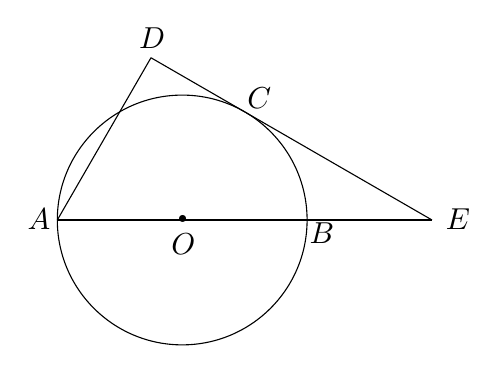
\begin{tikzpicture}[x=1pt, y=1pt,
    every node/.style={inner sep=0pt, font=\fontsize{10.5pt}{12.6pt}\selectfont}]

  % ---- 圆：m + 4c + h（源内容流 path 20，lw 0.398） ----
  % 源真页坐标：m (616.7234,353.2830)
  %   c (616.7234,328.3590) (596.5194,308.1550) (571.5954,308.1550)
  %   c (546.6714,308.1550) (526.4664,328.3590) (526.4664,353.2830)
  %   c (526.4664,378.2070) (546.6714,398.4110) (571.5954,398.4110)
  %   c (596.5194,398.4110) (616.7234,378.2070) (616.7234,353.2830)  h
  \draw[line width=0.398pt]
    (90.2570,45.1280)
    .. controls (90.2570,70.0520) and (70.0530,90.2560) .. (45.1290,90.2560)
    .. controls (20.2050,90.2560) and (0.0000,70.0520) .. (0.0000,45.1280)
    .. controls (0.0000,20.2040) and (20.2050,0.0000) .. (45.1290,0.0000)
    .. controls (70.0530,0.0000) and (90.2570,20.2040) .. (90.2570,45.1280)
    -- cycle;

  % ---- 垂线 AD（源 path 21，lw 0.398）：A(526.4672,353.2830) → D(560.3132,294.6600) ----
  \draw[line width=0.398pt] (0.0008,45.1280) -- (33.8468,103.7510);

  % ---- 直径延长线 AE（源 path 22，lw 0.398）：A(526.4672,353.2830) → E(661.8502,353.2830) ----
  \draw[line width=0.398pt] (0.0008,45.1280) -- (135.3838,45.1280);

  % ---- 切线 DE（源 path 23，lw 0.398）：D(560.3131,294.6605) → E(661.8501,353.2835) ----
  \draw[line width=0.398pt] (33.8467,103.7505) -- (135.3837,45.1275);

  % ---- 标签：源文本 Tm 原点（基线左端），CMMI10 10.5pt ----
  \node[anchor=base west] at (-10.9104,41.5400) {$A$};   % 源 (515.5560,356.8710)
  \node[anchor=base west] at (90.9416,36.6090)  {$B$};   % 源 (617.4080,361.8020)
  \node[anchor=base west] at (68.4956,85.5540)  {$C$};   % 源 (594.9620,312.8570)
  \node[anchor=base west] at (29.3546,107.1370) {$D$};   % 源 (555.8210,291.2740)
  \node[anchor=base west] at (140.1726,41.5400) {$E$};   % 源 (666.6390,356.8710)
  \node[anchor=base west] at (40.9786,32.5740)  {$O$};   % 源 (567.4450,365.8370)
  % 圆心点：源 CMSY10 0x0F（`\bullet`），Tm 为 0.6 缩放（CMSY10 10.5pt × 0.6），
  % 基线原点 (570.0200,354.6828) → 本地 (43.5536,43.7282)。
  \node[anchor=base west, scale=0.6] at (43.5536,43.7282) {$\bullet$};

\end{tikzpicture}
%
% 【自验结果】
%   探针：latexmk -pdfxe，0 error / 0 Overfull / 0 Underfull / 0 Missing character；
%         页面 162.34 × 114.08 pt（standalone border=0）。
%   tex 反算：4 条路径 + 7 个标签全部匹配，最大残差 0.000000 pt（阈值 0.05）。
%   600dpi 墨迹：整体墨迹包围盒最大边差 0.188 pt；几何包围盒 0.124 pt；
%         标签中心最大 0.240 pt（D）。（以上为尺度归一值，已扣除探针
%         0.996277 = 72/72.27 的 TeX pt / PDF bp 均匀因子）
%         按页面 bp 直接比较（物理）最大 0.604 pt，全部来自该 0.37% 均匀缩放。
%   灵敏度：端点 E +0.15pt → tex 检查器报 0.1500、600dpi 几何包围盒报 0.2409；
%         标签 C +0.15pt → tex 检查器报 0.1500、600dpi 标签中心报 0.1204。均能报出。
\end{center}
\nopagebreak[4]
\Needspace{4\baselineskip}
\textbf{解析}

\Needspace{5\baselineskip}
设 \(EB=e\)（\(e>0\)）。因 \(E\) 在 \(AB\) 的延长线上，故
\nopagebreak[4]
\[
EA=EB+BA=e+4.
\]
\Needspace{5\baselineskip}
由切割线定理，
\nopagebreak[4]
\[
CE^2=EB\cdot EA,
\]
\Needspace{5\baselineskip}
即
\nopagebreak[4]
\[
(2\sqrt3)^2=e(e+4).
\]
\Needspace{5\baselineskip}
展开得
\nopagebreak[4]
\[
e^2+4e-12=0,
\]
\Needspace{5\baselineskip}
解得 \(e=2\) 或 \(e=-6\)。因 \(e>0\)，故 \(e=2\)，从而
\nopagebreak[4]
\[
EA=6,\qquad OE=OB+BE=2+2=4.
\]

\Needspace{5\baselineskip}
连接 \(OC\)。因 \(EC\) 是圆 \(O\) 在 \(C\) 处的切线，故 \(OC\perp EC\)，且 \(OC=2\)。在直角三角形 \(OCE\) 中，
\nopagebreak[4]
\[
\sin\angle OEC=\dfrac{OC}{OE}=\dfrac{2}{4}=\dfrac12,
\]
\Needspace{5\baselineskip}
故 \(\angle OEC=30^\circ\)。由于 \(A\)，\(O\)，\(B\)，\(E\) 依次共线，射线 \(EA\) 与射线 \(EO\) 重合，所以
\nopagebreak[4]
\[
\angle AEC=\angle OEC=30^\circ.
\]
\Needspace{5\baselineskip}
又 \(AD\perp EC\)，即 \(AD\) 是点 \(A\) 到直线 \(EC\) 的距离，于是
\nopagebreak[4]
\[
AD=AE\sin\angle AEC=6\times\dfrac12=3.
\]

\Needspace{5\baselineskip}
（验证：以 \(O\) 为原点，\(x\) 轴沿 \(AB\) 方向，取 \(A(-2,0)\)，\(E(4,0)\)。切点 \(C(x,y)\) 满足 \(x^2+y^2=4\) 与 \(x(x-4)+y^2=0\)，两式相减得 \(x=1\)，从而 \(y=\sqrt3\)（取上半平面），此时 \(CE=2\sqrt3\)。直线 \(EC\) 的方程为 \(\sqrt3x+3y-4\sqrt3=0\)，点 \(A\) 到它的距离为
\nopagebreak[4]
\[
\dfrac{|-2\sqrt3-4\sqrt3|}{\sqrt{3+9}}=\dfrac{6\sqrt3}{2\sqrt3}=3,
\]
与所求一致。）

\gkanswer{答案：\(3\)}

\end{answer}
\begin{answer}
\gksolhead{16}{}

\textbf{题目}：

已知 \(\tan\alpha=2\)．

（1） 求 \(\tan\left(\alpha+\dfrac{\pi}{4}\right)\) 的值；

（2） 求 \(\dfrac{\sin 2\alpha}{\sin^2\alpha+\sin\alpha\cos\alpha-\cos 2\alpha-1}\) 的值．

\Needspace{4\baselineskip}
\textbf{解析}

已知 \(\tan\alpha=2\)，故 \(\cos\alpha\neq0\)，且 \(\sin\alpha=2\cos\alpha\)。

\gksubpart{(1)}

\Needspace{5\baselineskip}
由两角和的正切公式，并注意 \(\tan\dfrac{\pi}{4}=1\)，
\nopagebreak[4]
\[
\tan\left(\alpha+\dfrac{\pi}{4}\right)
=\dfrac{\tan\alpha+1}{1-\tan\alpha}
=\dfrac{2+1}{1-2}
=-3.
\]

\Needspace{5\baselineskip}
（验证：取 \(\cos\alpha=\dfrac{1}{\sqrt5}\)，\(\sin\alpha=\dfrac{2}{\sqrt5}\)，满足 \(\tan\alpha=2\)。则
\nopagebreak[4]
\[
\sin\left(\alpha+\dfrac{\pi}{4}\right)=\dfrac{1}{\sqrt2}\left(\dfrac{2}{\sqrt5}+\dfrac{1}{\sqrt5}\right)=\dfrac{3}{\sqrt{10}},
\]
\nopagebreak[4]
\[
\cos\left(\alpha+\dfrac{\pi}{4}\right)=\dfrac{1}{\sqrt2}\left(\dfrac{1}{\sqrt5}-\dfrac{2}{\sqrt5}\right)=-\dfrac{1}{\sqrt{10}},
\]
二者之比为 \(-3\)，与公式结果一致。）

\gksubpart{(2)}

\Needspace{5\baselineskip}
先化简分母。由 \(\cos2\alpha+1=2\cos^2\alpha\)，把分母中的 \(-\cos2\alpha-1\) 写成 \(-(\cos2\alpha+1)\)，得
\nopagebreak[4]
\[
\sin^2\alpha+\sin\alpha\cos\alpha-(\cos2\alpha+1)
=\sin^2\alpha+\sin\alpha\cos\alpha-2\cos^2\alpha.
\]
\Needspace{5\baselineskip}
因为 \(\cos\alpha\neq0\)，将分子分母同除以 \(\cos^2\alpha\)：
\nopagebreak[4]
\[
\dfrac{\sin2\alpha}{\sin^2\alpha+\sin\alpha\cos\alpha-2\cos^2\alpha}
=\dfrac{2\tan\alpha}{\tan^2\alpha+\tan\alpha-2}.
\]
\Needspace{5\baselineskip}
代入 \(\tan\alpha=2\)：
\nopagebreak[4]
\[
\dfrac{2\times2}{2^2+2-2}=\dfrac{4}{4}=1.
\]

\Needspace{5\baselineskip}
（验证：仍取 \(\sin\alpha=\dfrac{2}{\sqrt5}\)，\(\cos\alpha=\dfrac{1}{\sqrt5}\)。则 \(\sin^2\alpha=\dfrac45\)，\(\sin\alpha\cos\alpha=\dfrac25\)，\(\cos2\alpha=-\dfrac35\)，分子 \(\sin2\alpha=\dfrac45\)；分母为
\nopagebreak[4]
\[
\dfrac45+\dfrac25-\left(-\dfrac35\right)-1=\dfrac45,
\]
与分子相等，故比值为 \(1\)。）

\gkanswer{答案（1）：\(-3\)。}

\gkanswer{答案（2）：\(1\)。}

\end{answer}
\begin{answer}
\gksolhead{17}{}

\textbf{题目}：

某城市 100 户居民的月平均用电量（单位：度），以 \([160,180)\)，\([180,200)\)，\([200,220)\)，\([220,240)\)，\([240,260)\)，\([260,280)\)，\([280,300)\) 分组的频率分布直方图如图．
\nopagebreak[4]
\begin{center}% f2015gdw_q17_histogram.tex — 2015 年高考数学·广东卷·文科 第 17 题（频率分布直方图）
%
% 【来源】`.work/phase3-b16/source/2015广东文.pdf`（SHA-256
%   0c27f1a08f837014066c636a3190b8fa7ad7e5a4494f204e60412293aea17e09），
%   第 1 页（合订本页 949）第 3 栏；内容对象 5。逐路径实测见
%   `.work/phase3-b16/figure-inventory.md` Q17 节。
%
% 【坐标口径】清单坐标为「真页 pt、原点左上、y 向下」。本图取
%   X0 = 862.9140（y 轴 x），Y0 = 345.5480（x 轴基线 y_top），
%   本地坐标  (x, y) = (x_page − X0, Y0 − y_top)，
%   即本地原点 = 坐标轴交点，x 向右、y 向上，1 单位 = 1 TeX pt。
%   换算示例：原点 (862.9140,345.5479) → (0, 0.0001)；
%   柱 [160,180) 左边界 (885.5915,345.5485) → (22.6775,−0.0005)；
%   y 轴箭头尖 (862.9140,127.1584) → (0,218.3896)。
%   y 轴箭头的旋转坐标系按 PDF 行向量右乘（后写 cm 先作用）换算（FI-S5）。
%
% 【线宽/虚线】轴线与柱体 line width = 0.398pt；分式横线 0.42pt；
%   两枚箭头为填充路径（源 `f`，无描边；源 lw=1.0，填充路径下线宽不参与着色），
%   包围盒 2.99 × 3.99pt；依赖 \usetikzlibrary{arrows.meta}（按库规加载；
%   箭头用路径级贝塞尔复刻，未用 Triangle 造型）；
%   虚线导引线 dash pattern = on 2.989pt off 2.989pt，dash phase = 0pt。
%
% 【照源复刻的存疑项】
%   FI-S4：x 导引线 y_top=228.6168，[240,260) 柱顶 y_top=228.5026，
%          相差 0.1142pt；照录（导引线与柱顶分别定位）。
%   FI-S5：y 轴箭头在 `0 1 -1 0 862.914 711.14509 cm` 旋转坐标系内，
%          按行向量右乘解析，箭头包围盒 x 861.42–864.41、y_top 127.16–131.14。
%   FI-S8：底部 0.0025 / 0.002 基线仅差 7.85pt，照录。
%   FI-S10：x 轴 160…300 八个刻度在源内为单个 TJ 以字距排开，
%          此处按逐点 Tm 起点分别定位（起点取自 pdftotext -bbox）。
%   断轴三齿折线逐点照录（11 点；振幅 ±2.339pt）。
%
% 【自验结果】见文件末尾。
%
% 元素计数：18 条路径（轴+断轴 1、箭头 2、分式线 1、柱 7、虚线导引 7）、
%   21 个文本标签。
\begin{tikzpicture}[x=1pt, y=1pt,
    every node/.style={inner sep=0pt, font=\fontsize{10.5pt}{12.6pt}\selectfont}]

  % ---- y 轴 + 断轴 + x 轴（源 path 26，14 点折线，lw 0.398） ----
  % 源真页坐标：m (862.9140,130.7449) l (862.9140,345.5479) l (867.4490,345.5479)
  %   l (868.5830,343.2099) l (870.8510,347.8869) l (871.9850,345.5479)
  %   l (873.1190,343.2099) l (875.3870,347.8869) l (876.5210,345.5489)
  %   l (877.6550,343.2099) l (879.9230,347.8869) l (881.0570,345.5489)
  %   l (885.5920,345.5489) l (1086.1030,345.5479)
  \draw[line width=0.398pt]
    (0.0000,214.8031) -- (0.0000,0.0001)
    -- (4.5350,0.0001) -- (5.6690,2.3381) -- (7.9370,-2.3389)
    -- (9.0710,0.0001) -- (10.2050,2.3381) -- (12.4730,-2.3389)
    -- (13.6070,-0.0009) -- (14.7410,2.3381) -- (17.0090,-2.3389)
    -- (18.1430,-0.0009) -- (22.6780,-0.0009) -- (223.1890,0.0001);

  % ---- y 轴箭头（源 path 27，两段贝塞尔，填充，无描边） ----
  % 源真页坐标（FI-S5 校正后）：尖 (862.9140,127.1584)
  %   c (862.7150,128.2214) (862.1170,129.9484) (861.4200,131.1434)
  %   l (864.4080,131.1434)
  %   c (863.7110,129.9484) (863.1130,128.2214) (862.9140,127.1584)
  \fill[line width=1.0pt]
    (0.0000,218.3896)
    .. controls (-0.1990,217.3266) and (-0.7970,215.5996) .. (-1.4940,214.4046)
    -- (1.4940,214.4046)
    .. controls (0.7970,215.5996) and (0.1990,217.3266) .. (0.0000,218.3896)
    -- cycle;

  % ---- x 轴箭头（源 path 28，两段贝塞尔，填充，无描边） ----
  % 源真页坐标：尖 (1089.6893,345.5480)
  %   c (1088.6263,345.3490) (1086.8993,344.7510) (1085.7043,344.0540)
  %   l (1085.7043,347.0420)
  %   c (1086.8993,346.3450) (1088.6263,345.7470) (1089.6893,345.5480)
  \fill[line width=1.0pt]
    (226.7753,0.0000)
    .. controls (225.7123,0.1990) and (223.9853,0.7970) .. (222.7903,1.4940)
    -- (222.7903,-1.4940)
    .. controls (223.9853,-0.7970) and (225.7123,-0.1990) .. (226.7753,0.0000)
    -- cycle;

  % ---- 「频率/组距」分式横线（源 path 29，lw 0.42） ----
  % 源真页坐标：(867.8080,127.8390) → (888.8080,127.8390)
  \draw[line width=0.42pt] (4.8940,217.7090) -- (25.8940,217.7090);

  % ---- 柱 [160,180)：源 path 30，m,l,l,l,h，lw 0.398 ----
  \draw[line width=0.398pt]
    (22.6775,31.1645) -- (22.6775,-0.0005) -- (45.3555,-0.0005)
    -- (45.3555,31.1645) -- cycle;
  % ---- 导引线 0.002：源 path 31，虚线 ----
  \draw[line width=0.398pt, dash pattern=on 2.989pt off 2.989pt, dash phase=0pt]
    (0.0000,31.1645) -- (22.6780,31.1645);

  % ---- 柱 [180,200)：源 path 32 ----
  \draw[line width=0.398pt]
    (45.3551,148.2099) -- (45.3551,-0.0001) -- (68.0331,-0.0001)
    -- (68.0331,148.2099) -- cycle;
  % ---- 导引线 0.0095：源 path 33 ----
  \draw[line width=0.398pt, dash pattern=on 2.989pt off 2.989pt, dash phase=0pt]
    (0.0000,148.2099) -- (45.3550,148.2099);

  % ---- 柱 [200,220)：源 path 34 ----
  \draw[line width=0.398pt]
    (68.0326,171.5239) -- (68.0326,-0.0001) -- (90.7106,-0.0001)
    -- (90.7106,171.5239) -- cycle;
  % ---- 导引线 0.011：源 path 35 ----
  \draw[line width=0.398pt, dash pattern=on 2.989pt off 2.989pt, dash phase=0pt]
    (0.0000,171.5239) -- (68.0330,171.5239);

  % ---- 柱 [220,240)：源 path 36 ----
  \draw[line width=0.398pt]
    (90.7101,194.8378) -- (90.7101,-0.0002) -- (113.3881,-0.0002)
    -- (113.3881,194.8378) -- cycle;
  % ---- 导引线 0.0125：源 path 37 ----
  \draw[line width=0.398pt, dash pattern=on 2.989pt off 2.989pt, dash phase=0pt]
    (0.0000,194.8378) -- (90.7100,194.8378);

  % ---- 柱 [240,260)：源 path 38（注意本柱顶无独立导引线，见 FI-S4） ----
  \draw[line width=0.398pt]
    (113.3877,117.0454) -- (113.3877,0.0004) -- (136.0657,0.0004)
    -- (136.0657,117.0454) -- cycle;

  % ---- 柱 [260,280)：源 path 39 ----
  \draw[line width=0.398pt]
    (136.0652,78.0303) -- (136.0652,0.0003) -- (158.7432,0.0003)
    -- (158.7432,78.0303) -- cycle;
  % ---- 导引线 0.005：源 path 40 ----
  \draw[line width=0.398pt, dash pattern=on 2.989pt off 2.989pt, dash phase=0pt]
    (0.0000,78.0303) -- (136.0650,78.0303);

  % ---- 柱 [280,300)：源 path 41 ----
  \draw[line width=0.398pt]
    (158.7427,39.0151) -- (158.7427,0.0001) -- (181.4207,0.0001)
    -- (181.4207,39.0151) -- cycle;
  % ---- 导引线 0.0025：源 path 42 ----
  \draw[line width=0.398pt, dash pattern=on 2.989pt off 2.989pt, dash phase=0pt]
    (0.0000,39.0151) -- (158.7430,39.0151);

  % ---- 导引线 x：源 path 43（y_top 228.6168，与柱顶差 0.1142pt，FI-S4） ----
  \draw[line width=0.398pt, dash pattern=on 2.989pt off 2.989pt, dash phase=0pt]
    (0.0000,116.9312) -- (113.3880,116.9312);

  % ---- 文本标签：源 Tm/Td 基线原点，10.5pt ----
  % 「频率/组距」：STSong；源基线 (867.8080,123.3610) / (867.8080,137.6670)
  \node[anchor=base west] at (4.8940,222.1870) {频率};
  \node[anchor=base west] at (4.8940,207.8810) {组距};
  % y 轴刻度值（源 C0_1 LMRoman10；基线左端）
  \node[anchor=base west] at (-32.8680,191.4570) {$0.0125$};  % 源 (830.0460,154.0910)
  \node[anchor=base west] at (-27.6180,168.1430) {$0.011$};   % 源 (835.2960,177.4050)
  \node[anchor=base west] at (-32.8680,144.8290) {$0.0095$};  % 源 (830.0460,200.7190)
  \node[anchor=base west] at (-9.7000,114.6710)  {$x$};       % 源 (853.2140,230.8770) CMMI10
  \node[anchor=base west] at (-27.6180,74.6490)  {$0.005$};   % 源 (835.2960,270.8990)
  \node[anchor=base west] at (-32.8680,35.6340)  {$0.0025$};  % 源 (830.0460,309.9140)
  \node[anchor=base west] at (-27.6180,27.7830)  {$0.002$};   % 源 (835.2960,317.7650)
  % 原点 0（源 (860.2890,356.2400)）
  \node[anchor=base west] at (-2.6250,-10.6920) {$0$};
  % x 轴刻度（源为单个 TJ；以下为逐点 Tm 起点，基线 y_top=356.0140）
  \node[anchor=base west] at (14.8020,-10.4660)  {$160$};  % 源 (877.716000,356.014)
  \node[anchor=base west] at (37.4800,-10.4660)  {$180$};  % 源 (900.394005,356.014)
  \node[anchor=base west] at (60.1570,-10.4660)  {$200$};  % 源 (923.071002,356.014)
  \node[anchor=base west] at (82.8350,-10.4660)  {$220$};  % 源 (945.749007,356.014)
  \node[anchor=base west] at (105.5130,-10.4660) {$240$};  % 源 (968.427012,356.014)
  \node[anchor=base west] at (128.1900,-10.4660) {$260$};  % 源 (991.104009,356.014)
  \node[anchor=base west] at (150.8680,-10.4660) {$280$};  % 源 (1013.782014,356.014)
  \node[anchor=base west] at (173.5450,-10.4660) {$300$};  % 源 (1036.459011,356.014)
  % x 轴标题「月平均用电量/度」：源三段分别定位，同一基线 (…,339.2240)
  \node[anchor=base west] at (187.4000,6.3240) {月平均用电量};  % 源 (1050.3140,339.2240) STSong
  \node[anchor=base west] at (250.4000,6.3240) {/};             % 源 (1113.3140,339.2240) LMRoman10
  \node[anchor=base west] at (255.6500,6.3240) {度};            % 源 (1118.5640,339.2240) STSong

\end{tikzpicture}
%
% 【自验结果】
%   探针：latexmk -pdfxe，0 error / 0 Overfull / 0 Underfull / 0 Missing character；
%         页面 301.40 × 240.11 pt（standalone border=0）。
%   tex 反算：18 条路径 + 21 个标签全部匹配，最大残差 0.000020 pt（阈值 0.05）。
%   600dpi 墨迹：整体墨迹包围盒最大边差 0.278 pt；几何包围盒 0.213 pt；
%         标签中心最大 0.273 pt（280）。（尺度归一，已扣除 0.996277 的
%         TeX pt / PDF bp 均匀因子）
%         按页面 bp 直接比较（物理）最大 0.952 pt（几何包围盒），来自该 0.37% 均匀缩放。
%   灵敏度：y 轴线宽 +0.02pt → 600dpi 等效线宽 +0.0358（tex 检查器不检线宽，报 0）；
%         刻度 200 y +0.15pt → tex 检查器报 0.1500、600dpi 标签中心报 0.2409。均能报出。
\end{center}
\nopagebreak[4]
（1） 求直方图中 \(x\) 的值；

（2） 求月平均用电量的众数和中位数；

（3） 在月平均用电量为 \([220,240)\)，\([240,260)\)，\([260,280)\)，\([280,300)\) 的四组用户中，用分层抽样的方法抽取 11 户居民，则月平均用电量在 \([220,240)\) 的用户中应抽取多少户？

\Needspace{4\baselineskip}
\textbf{解析}

由直方图读出各组的 \(\dfrac{\text{频率}}{\text{组距}}\)：\([160,180)\) 为 \(0.002\)，\([180,200)\) 为 \(0.0095\)，\([200,220)\) 为 \(0.011\)，\([220,240)\) 为 \(0.0125\)，\([240,260)\) 为 \(x\)，\([260,280)\) 为 \(0.005\)，\([280,300)\) 为 \(0.0025\)。各组组距均为 \(20\)。

\gksubpart{(1)}

\Needspace{5\baselineskip}
直方图中所有矩形的面积之和为 \(1\)，即
\nopagebreak[4]
\[
20\,(0.002+0.0095+0.011+0.0125+x+0.005+0.0025)=1.
\]
\Needspace{5\baselineskip}
括号内不含 \(x\) 的各项之和为
\nopagebreak[4]
\[
0.002+0.0095+0.011+0.0125+0.005+0.0025=0.0425,
\]
\Needspace{5\baselineskip}
故
\nopagebreak[4]
\[
20\,(0.0425+x)=1
\;\Longrightarrow\;
0.0425+x=0.05
\;\Longrightarrow\;
x=0.0075.
\]

（验证：将 \(x=0.0075\) 代回，柱高之和为 \(0.05\)，总面积 \(20\times0.05=1\)，归一化成立。按图中导引线与柱高两种读法折算，分别得 \(0.00750\) 与 \(0.00751\)，均与计算值 \(0.0075\) 一致。）

\gksubpart{(2)}

\Needspace{5\baselineskip}
各组频率等于柱高乘以组距 \(20\)，依次为
\nopagebreak[4]
\[
0.04,\quad0.19,\quad0.22,\quad0.25,\quad0.15,\quad0.10,\quad0.05.
\]
\Needspace{5\baselineskip}
其中最高的矩形是 \([220,240)\)，故众数取该组底边中点：
\nopagebreak[4]
\[
\dfrac{220+240}{2}=230.
\]

\Needspace{5\baselineskip}
累计频率依次为
\nopagebreak[4]
\[
0.04,\quad0.23,\quad0.45,\quad0.70,\quad0.85,\quad0.95,\quad1.
\]
\Needspace{5\baselineskip}
因 \(0.45<0.5<0.70\)，中位数位于 \([220,240)\) 内。设中位数为 \(220+t\)（\(0<t<20\)），由该组内频率均匀分布，
\nopagebreak[4]
\[
0.45+\dfrac{t}{20}\times0.25=0.5,
\]
解得 \(t=4\)，故中位数为 \(224\)。

（验证：中位数左侧面积为 \(0.45+\dfrac{4}{20}\times0.25=0.50\)；右侧面积为 \(\dfrac{16}{20}\times0.25+0.15+0.10+0.05=0.20+0.30=0.50\)，左右各半。）

\gksubpart{(3)}

\Needspace{5\baselineskip}
四组 \([220,240)\)，\([240,260)\)，\([260,280)\)，\([280,300)\) 的频率分别为
\nopagebreak[4]
\[
0.25,\quad0.15,\quad0.10,\quad0.05,
\]
合计 \(0.55\)。样本容量为 \(100\)，故四组户数依次为 \(25\)，\(15\)，\(10\)，\(5\)，共 \(55\) 户。

\Needspace{5\baselineskip}
分层抽样抽取 \(11\) 户，抽样比为
\nopagebreak[4]
\[
\dfrac{11}{55}=\dfrac15.
\]
\Needspace{5\baselineskip}
故 \([220,240)\) 组应抽取
\nopagebreak[4]
\[
25\times\dfrac15=5\ \text{户}.
\]

（验证：各组抽取数依次为 \(25\times\dfrac15=5\)，\(15\times\dfrac15=3\)，\(10\times\dfrac15=2\)，\(5\times\dfrac15=1\)，合计 \(5+3+2+1=11\)，与抽取总数吻合。）

\gkanswer{答案（1）：\(x=0.0075\)。}

\gkanswer{答案（2）：众数 \(230\)（度），中位数 \(224\)（度）。}

\gkanswer{答案（3）：\(5\) 户。}

\end{answer}
\begin{answer}
\gksolhead{18}{}

\textbf{题目}：

如图，三角形 \(PDC\) 所在的平面与长方形 \(ABCD\) 所在的平面垂直，\(PD=PC=4\)，\(AB=6\)，\(BC=3\)．
\nopagebreak[4]
\begin{center}% f2015gdw_q18_solid.tex — 2015 年高考数学·广东卷·文科 第 18 题（四棱锥 P-ABCD 立体图）
%
% 【来源】`.work/phase3-b16/source/2015广东文.pdf`
%   （SHA-256 0c27f1a08f837014066c636a3190b8fa7ad7e5a4494f204e60412293aea17e09），
%   第 2 页（合订本页 950）第 1 栏；内容对象 20。逐路径实测见
%   `.work/phase3-b16/figure-inventory.md` Q18 节。
%
% 【坐标口径】清单坐标为「真页 pt、原点左上、y 向下」。本图取
%   X0 = 202.0221（顶点 A 的 x），Y0 = 274.11714（顶点 A 的 y_top），
%   本地坐标  (x, y) = (x_page − X0, Y0 − y_top)，
%   即本地原点 = 顶点 A，x 向右、y 向上，1 单位 = 1 TeX pt。
%   换算示例：A (202.0221,274.1171) → (0,0)；B (365.2908,274.1171) → (163.2687,0)；
%   C (389.7813,233.3000) → (187.7592,40.8171)；D (226.5127,233.3000) → (24.4906,40.8171)；
%   P (308.1470,161.3053) → (106.1249,112.8119)。
%
% 【线宽/虚线】全部棱 line width = 0.3985pt（源先写 0.59776 w 随即被 0.3985 w 覆盖）；
%   DC 短段 dash pattern = on 2.98883pt off 2.98883pt，dash phase = 0pt；
%   无填充、无 c 算子（全为 m/l 直线）。
%
% 【照源复刻的存疑项】
%   FI-S1：DC 自 D 起为虚线，虚线终点 x=240.1184（∩ PA 计算值 x≈240.42，
%          差 0.30pt）；虚线路径方向照源为「交点 → D」，相位 0 起于交点。
%   FI-S2：源未画棱 PB，照录不补。
%   FI-S3：源每条棱路径起点有零长度重复 moveto（共 8 处），按规范不复刻。
%   FI-S9：Q18(1) 的「∥」在正文行内（y_top 89.20–98.25），不属于图形区，
%          不在本图内绘制。
%
% 【自验结果】见文件末尾。
%
% 元素计数：8 条棱（PA / PC / PD / DA / AB / BC / DC 实线 + DC 虚线）、5 个标签。
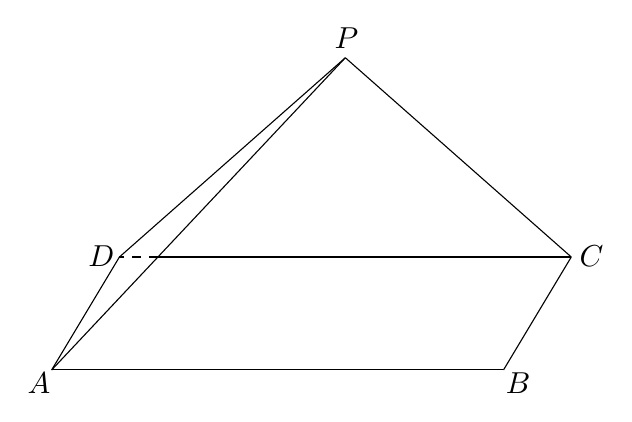
\begin{tikzpicture}[x=1pt, y=1pt,
    every node/.style={inner sep=0pt, font=\fontsize{10.5pt}{12.6pt}\selectfont}]

  % ---- 顶点（本地坐标） ----
  % A (0,0)  B (163.2687,0)  C (187.7592,40.8171)  D (24.4906,40.8171)  P (106.1249,112.8119)

  % ---- P–A（源 path 11：m A(202.0221,274.1171) l P(308.1470,161.3053)，本图反向） ----
  \draw[line width=0.3985pt] (106.1249,112.8119) -- (0.0000,0.0000);

  % ---- P–C（源 m (308.1470,161.3053) l (389.7813,233.3000)） ----
  \draw[line width=0.3985pt] (106.1249,112.8119) -- (187.7592,40.8171);

  % ---- P–D（源 path 3：m D(226.5127,233.3000) l P(308.1470,161.3053)，本图反向） ----
  \draw[line width=0.3985pt] (106.1249,112.8119) -- (24.4906,40.8171);

  % ---- D–A（源 path 7：m A(202.0221,274.1171) l D(226.5127,233.3000)，本图反向） ----
  \draw[line width=0.3985pt] (24.4906,40.8171) -- (0.0000,0.0000);

  % ---- A–B（源 path 9：m B(365.2908,274.1171) l A(202.0221,274.1171)，本图反向） ----
  \draw[line width=0.3985pt] (0.0000,0.0000) -- (163.2687,0.0000);

  % ---- B–C（源 m (365.2908,274.1171) l (389.7813,233.3000)） ----
  \draw[line width=0.3985pt] (163.2687,0.0000) -- (187.7592,40.8171);

  % ---- D–C 实线段（源 m (389.7813,233.3000) l (240.1184,233.3000)） ----
  \draw[line width=0.3985pt] (187.7592,40.8171) -- (38.0963,40.8171);

  % ---- D–C 虚线段（源 m (240.1184,233.3000) l (226.5127,233.3000)，方向照源） ----
  \draw[line width=0.3985pt, dash pattern=on 2.98883pt off 2.98883pt, dash phase=0pt]
    (38.0963,40.8171) -- (24.4906,40.8171);

  % ---- 标签：源文本 Tm 原点（基线左端），CMMI10 10.5pt ----
  \node[anchor=base west] at (102.0249,116.1981) {$P$};  % 源 (304.0470,157.9190)
  \node[anchor=base west] at (13.0239,37.2291)   {$D$};  % 源 (215.0460,236.8880)
  \node[anchor=base west] at (190.6049,37.2291)  {$C$};  % 源 (392.6270,236.8880)
  \node[anchor=base west] at (-8.8691,-8.5189)   {$A$};  % 源 (193.1530,282.6360)
  \node[anchor=base west] at (163.9539,-8.5189)  {$B$};  % 源 (365.9760,282.6360)

\end{tikzpicture}
%
% 【自验结果】
%   探针：latexmk -pdfxe，0 error / 0 Overfull / 0 Underfull / 0 Missing character；
%         页面 210.45 × 131.40 pt（standalone border=0）。
%   tex 反算：8 条棱 + 5 个标签全部匹配，最大残差 0.000057 pt（阈值 0.05）。
%   600dpi 墨迹：整体墨迹包围盒最大边差 0.285 pt；几何包围盒 0.064 pt；
%         标签中心最大 0.255 pt（C）。（尺度归一，已扣除 0.996277 的
%         TeX pt / PDF bp 均匀因子）
%         按页面 bp 直接比较（物理）最大 0.695 pt，来自该 0.37% 均匀缩放。
%   灵敏度：顶点 C x +0.15pt → tex 检查器报 0.1500、600dpi 几何包围盒报 0.1204。能报出。
\end{center}
\nopagebreak[4]
（1） 证明：\(BC\parallel\) 平面 \(PDA\)；

（2） 证明：\(BC\perp PD\)；

（3） 求点 \(C\) 到平面 \(PDA\) 的距离．

\Needspace{4\baselineskip}
\textbf{解析}

\gksubpart{(1)}

因为 \(ABCD\) 是长方形，所以 \(BC\parallel AD\)。

由 \(PD=PC=4\)，\(DC=AB=6\)，点 \(P\) 不在直线 \(DC\) 上（否则 \(PD+PC=DC\) 或 \(|PD-PC|=DC\)，均与已知矛盾）。而平面 \(PDC\) 与平面 \(ABCD\) 的交线为 \(DC\)，故 \(P\notin\text{平面 }ABCD\)。于是平面 \(PDA\) 与平面 \(ABCD\) 不重合，它们有公共点 \(A\)、\(D\)，故交线为 \(AD\)。因 \(B\notin AD\)，所以 \(B\notin\text{平面 }PDA\)，即 \(BC\not\subset\text{平面 }PDA\)。

\Needspace{5\baselineskip}
又 \(AD\subset\text{平面 }PDA\)，由线面平行的判定定理，
\nopagebreak[4]
\[
BC\parallel\text{平面}\ PDA.
\]

（验证：用第 (3) 问的坐标系，\(\overrightarrow{BC}=(0,-3,0)\)，平面 \(PDA\) 的法向量为 \((3\sqrt7,0,-9)\)，二者点积为 \(0\)；又 \(B(6,3,0)\) 代入平面方程 \(\sqrt7x-3z=0\) 得 \(6\sqrt7\neq0\)，即 \(B\notin\text{平面 }PDA\)。方向平行且直线不在平面内，与判定定理一致。）

\gksubpart{(2)}

在长方形 \(ABCD\) 中，\(BC\perp DC\)。

\Needspace{5\baselineskip}
因为平面 \(PDC\perp\text{平面 }ABCD\)，且交线为 \(DC\)，\(BC\subset\text{平面 }ABCD\)，\(BC\perp DC\)，由面面垂直的性质定理得
\nopagebreak[4]
\[
BC\perp\text{平面}\ PDC.
\]
\Needspace{5\baselineskip}
又 \(PD\subset\text{平面 }PDC\)，所以
\nopagebreak[4]
\[
BC\perp PD.
\]

（验证：用第 (3) 问的坐标系，\(\overrightarrow{BC}=(0,-3,0)\)，\(\overrightarrow{PD}=(-3,0,-\sqrt7)\)，点积为 \(0\times(-3)+(-3)\times0+0\times(-\sqrt7)=0\)，故 \(BC\perp PD\)，与几何证明一致。）

\gksubpart{(3)}

\Needspace{5\baselineskip}
取 \(DC\) 的中点 \(M\)，连接 \(PM\)。由 \(PD=PC=4\)，\(DC=6\) 得 \(DM=3\)，且 \(PM\perp DC\)，所以
\nopagebreak[4]
\[
PM=\sqrt{PD^2-DM^2}=\sqrt{16-9}=\sqrt7.
\]
因为平面 \(PDC\perp\text{平面 }ABCD\)，交线为 \(DC\)，\(PM\subset\text{平面 }PDC\) 且 \(PM\perp DC\)，所以 \(PM\perp\text{平面 }ABCD\)。

\Needspace{5\baselineskip}
以 \(D\) 为原点，\(DC\) 所在直线为 \(x\) 轴，\(DA\) 所在直线为 \(y\) 轴，过 \(D\) 且垂直于平面 \(ABCD\) 向上的方向为 \(z\) 轴正方向，建立空间直角坐标系，则
\nopagebreak[4]
\[
D(0,0,0),\quad C(6,0,0),\quad A(0,3,0),\quad B(6,3,0),\quad P(3,0,\sqrt7).
\]
\Needspace{5\baselineskip}
于是
\nopagebreak[4]
\[
\overrightarrow{DA}=(0,3,0),\qquad \overrightarrow{DP}=(3,0,\sqrt7),
\]
\Needspace{5\baselineskip}
平面 \(PDA\) 的一个法向量为
\nopagebreak[4]
\[
\vec n=\overrightarrow{DA}\times\overrightarrow{DP}=(3\sqrt7,0,-9).
\]
\Needspace{5\baselineskip}
平面 \(PDA\) 过原点 \(D\)，其方程为
\nopagebreak[4]
\[
3\sqrt7\,x-9z=0,\quad\text{即}\quad \sqrt7\,x-3z=0.
\]
\Needspace{5\baselineskip}
点 \(C(6,0,0)\) 到平面 \(PDA\) 的距离为
\nopagebreak[4]
\[
d=\dfrac{|6\sqrt7|}{\sqrt{(\sqrt7)^2+(-3)^2}}=\dfrac{6\sqrt7}{4}=\dfrac{3\sqrt7}{2}.
\]

（验证：体积法。\(PM\perp\text{平面 }ACD\)，\(S_{\triangle ACD}=\dfrac12\cdot AD\cdot DC=9\)，故 \(V_{P-ACD}=\dfrac13\cdot9\cdot\sqrt7=3\sqrt7\)。又 \(DA=3\)，\(DP=4\)，\(PA=\sqrt{3^2+3^2+7}=5\)，有 \(DA^2+DP^2=PA^2\)，所以 \(S_{\triangle PDA}=\dfrac12\cdot3\cdot4=6\)。于是 \(d=\dfrac{3V_{P-ACD}}{S_{\triangle PDA}}=\dfrac{9\sqrt7}{6}=\dfrac{3\sqrt7}{2}\approx3.969\)，与坐标法结果一致。）

\gkanswer{答案（1）：成立（长方形 \(ABCD\) 中 \(BC\parallel AD\)，\(AD\subset\) 平面 \(PDA\)，\(BC\not\subset\) 平面 \(PDA\)，故 \(BC\parallel\) 平面 \(PDA\)）。}

\gkanswer{答案（2）：成立（平面 \(PDC\perp\) 平面 \(ABCD\)，交线为 \(DC\)；\(BC\perp DC\)，故 \(BC\perp\) 平面 \(PDC\)，从而 \(BC\perp PD\)）。}

\gkanswer{答案（3）：\(\dfrac{3\sqrt{7}}{2}\)。}

\end{answer}
\begin{answer}
\gksolhead{19}{}

\textbf{题目}：

设数列 \(\{a_n\}\) 的前 \(n\) 项和为 \(S_n\)，\(n\in\mathbf{N}^{*}\)，已知 \(a_1=1\)，\(a_2=\dfrac{3}{2}\)，\(a_3=\dfrac{5}{4}\)，且当 \(n\geqslant 2\) 时，\(4S_{n+2}+5S_n=8S_{n+1}+S_{n-1}\)．

（1） 求 \(a_4\) 的值；

（2） 证明：\(\left\{a_{n+1}-\dfrac{1}{2}a_n\right\}\) 为等比数列；

（3） 求数列 \(\{a_n\}\) 的通项公式．

\Needspace{4\baselineskip}
\textbf{解析}

\gksubpart{(1)}

\Needspace{5\baselineskip}
由 \(a_1=1\)，\(a_2=\dfrac32\)，\(a_3=\dfrac54\) 得
\nopagebreak[4]
\[
S_1=1,\qquad S_2=1+\dfrac32=\dfrac52,\qquad S_3=\dfrac52+\dfrac54=\dfrac{15}{4}.
\]
\Needspace{5\baselineskip}
在 \(4S_{n+2}+5S_n=8S_{n+1}+S_{n-1}\)（\(n\geqslant2\)）中取 \(n=2\)：
\nopagebreak[4]
\[
4S_4+5S_2=8S_3+S_1,
\]
\Needspace{5\baselineskip}
即
\nopagebreak[4]
\[
4S_4=8\cdot\dfrac{15}{4}+1-5\cdot\dfrac52=30+1-\dfrac{25}{2}=\dfrac{37}{2},
\]
\Needspace{5\baselineskip}
故 \(S_4=\dfrac{37}{8}\)，从而
\nopagebreak[4]
\[
a_4=S_4-S_3=\dfrac{37}{8}-\dfrac{15}{4}=\dfrac78.
\]

（验证：把 \(S_4=\dfrac{37}{8}\) 代回 \(n=2\) 时的递推式，左边 \(=4\cdot\dfrac{37}{8}+5\cdot\dfrac52=\dfrac{37}{2}+\dfrac{25}{2}=31\)，右边 \(=8\cdot\dfrac{15}{4}+1=31\)，两端相等。）

\gksubpart{(2)}

\Needspace{5\baselineskip}
当 \(n\geqslant2\) 时，已知
\nopagebreak[4]
\[
4S_{n+2}+5S_n=8S_{n+1}+S_{n-1}. \tag*{(i)}
\]
\Needspace{5\baselineskip}
将 \(n\) 换成 \(n+1\)（此时 \(n\geqslant1\)），得
\nopagebreak[4]
\[
4S_{n+3}+5S_{n+1}=8S_{n+2}+S_n. \tag*{(ii)}
\]
\Needspace{5\baselineskip}
(ii) 减 (i)（\(n\geqslant2\)），并利用 \(S_{k+1}-S_k=a_{k+1}\)，得
\nopagebreak[4]
\[
4a_{n+3}+5a_{n+1}=8a_{n+2}+a_n. \tag*{(iii)}
\]
\Needspace{5\baselineskip}
将 (iii) 移项整理为
\nopagebreak[4]
\[
4a_{n+3}-4a_{n+2}+a_{n+1}=4a_{n+2}-4a_{n+1}+a_n. \tag*{(iv)}
\]
\Needspace{5\baselineskip}
令 \(d_n=4a_{n+2}-4a_{n+1}+a_n\)，则 (iv) 即
\nopagebreak[4]
\[
d_{n+1}=d_n\quad(n\geqslant2).
\]
\Needspace{5\baselineskip}
计算
\nopagebreak[4]
\[
d_1=4a_3-4a_2+a_1=5-6+1=0,
\]
\nopagebreak[4]
\[
d_2=4a_4-4a_3+a_2=4\cdot\dfrac78-4\cdot\dfrac54+\dfrac32=\dfrac72-5+\dfrac32=0.
\]
\Needspace{5\baselineskip}
所以 \(d_n=0\) 对一切 \(n\geqslant1\) 成立，即
\nopagebreak[4]
\[
4a_{n+2}-4a_{n+1}+a_n=0,
\]
\Needspace{5\baselineskip}
亦即
\nopagebreak[4]
\[
a_{n+2}-\dfrac12a_{n+1}=\dfrac12\left(a_{n+1}-\dfrac12a_n\right).
\]
\Needspace{5\baselineskip}
令 \(b_n=a_{n+1}-\dfrac12a_n\)，则 \(b_{n+1}=\dfrac12b_n\)，且
\nopagebreak[4]
\[
b_1=a_2-\dfrac12a_1=\dfrac32-\dfrac12=1\neq0.
\]
故 \(\{b_n\}\) 是首项为 \(1\)、公比为 \(\dfrac12\) 的等比数列。

（验证：逐项计算 \(b_1=1\)，\(b_2=a_3-\dfrac12a_2=\dfrac54-\dfrac34=\dfrac12\)，\(b_3=a_4-\dfrac12a_3=\dfrac78-\dfrac58=\dfrac14\)，相邻项之比均为 \(\dfrac12\)，与首项 \(1\)、公比 \(\dfrac12\) 吻合。）

\gksubpart{(3)}

\Needspace{5\baselineskip}
由 (2) 得
\nopagebreak[4]
\[
b_n=a_{n+1}-\dfrac12a_n=\left(\dfrac12\right)^{n-1}.
\]
\Needspace{5\baselineskip}
两边同乘 \(2^n\)：
\nopagebreak[4]
\[
2^na_{n+1}-2^{n-1}a_n=2.
\]
\Needspace{5\baselineskip}
令 \(c_n=2^{n-1}a_n\)，则 \(c_{n+1}-c_n=2\)，且 \(c_1=2^0a_1=1\)。所以 \(\{c_n\}\) 是首项为 \(1\)、公差为 \(2\) 的等差数列，
\nopagebreak[4]
\[
c_n=1+2(n-1)=2n-1,
\]
\Needspace{5\baselineskip}
从而
\nopagebreak[4]
\[
a_n=\dfrac{c_n}{2^{n-1}}=\dfrac{2n-1}{2^{n-1}}.
\]

（验证：由递推式逐项迭代得 \(a_1,a_2,a_3,a_4,a_5=1,\dfrac32,\dfrac54,\dfrac78,\dfrac9{16}\)，公式 \(a_n=\dfrac{2n-1}{2^{n-1}}\) 在 \(n=1,2,3,4,5\) 处给出相同数值。再取 \(n=3\) 检查原递推式：左边 \(=4S_5+5S_3=4\cdot\dfrac{83}{16}+5\cdot\dfrac{15}{4}=\dfrac{83}{4}+\dfrac{75}{4}=\dfrac{79}{2}\)，右边 \(=8S_4+S_2=8\cdot\dfrac{37}{8}+\dfrac52=\dfrac{79}{2}\)，两端相等。）

\gkanswer{答案（1）：\(a_4=\dfrac{7}{8}\)。}

\gkanswer{答案（2）：成立（\(\left\{a_{n+1}-\dfrac{1}{2}a_n\right\}\) 是首项为 \(1\)、公比为 \(\dfrac{1}{2}\) 的等比数列）。}

\gkanswer{答案（3）：\(a_n=\dfrac{2n-1}{2^{n-1}}\)。}

\end{answer}
\begin{answer}
\gksolhead{20}{}

\textbf{题目}：

已知过原点的动直线 \(l\) 与圆 \(C_1: x^2+y^2-6x+5=0\) 相交于不同的两点 \(A\)，\(B\)．

（1） 求圆 \(C_1\) 的圆心坐标；

（2） 求线段 \(AB\) 的中点 \(M\) 的轨迹 \(C\) 的方程；

（3） 是否存在实数 \(k\)，使得直线 \(L: y=k(x-4)\) 与曲线 \(C\) 只有一个交点？若存在，求出 \(k\) 的取值范围；若不存在，说明理由．

\Needspace{4\baselineskip}
\textbf{解析}

\gksubpart{(1)}

\Needspace{5\baselineskip}
将圆 \(C_1\) 的方程配方：
\nopagebreak[4]
\[
x^2+y^2-6x+5=0\iff (x-3)^2+y^2=4.
\]
故圆 \(C_1\) 的圆心为 \(C_1(3,0)\)，半径为 \(2\)。

（验证：展开 \((x-3)^2+y^2=4\) 得 \(x^2-6x+9+y^2=4\)，即 \(x^2+y^2-6x+5=0\)，与原方程一致，故圆心 \((3,0)\)、半径 \(2\) 正确。）

\gksubpart{(2)}

\Needspace{5\baselineskip}
设 \(M(x,y)\)。因为 \(M\) 是弦 \(AB\) 的中点，所以 \(C_1M\perp AB\)。又 \(A\)、\(B\)、\(M\) 都在过原点 \(O\) 的直线 \(l\) 上，所以 \(OM\) 与 \(l\) 同向，从而
\nopagebreak[4]
\[
C_1M\perp OM.
\]
\Needspace{5\baselineskip}
用坐标表示：
\nopagebreak[4]
\[
(x-3,\ y)\cdot(x,\ y)=0,
\]
\Needspace{5\baselineskip}
即
\nopagebreak[4]
\[
x^2+y^2-3x=0,
\]
\Needspace{5\baselineskip}
配方得
\nopagebreak[4]
\[
\left(x-\dfrac32\right)^2+y^2=\dfrac94. \tag*{(v)}
\]
这就是以 \(OC_1\) 为直径的圆。

\Needspace{5\baselineskip}
确定范围。由 (v) 得 \(x^2+y^2=3x\)，于是
\nopagebreak[4]
\[
y^2=3x-x^2\geqslant0\implies 0\leqslant x\leqslant3.
\]
\Needspace{5\baselineskip}
设圆心 \(C_1\) 到直线 \(l\) 的距离为 \(d\)。因为 \(l\) 与圆有两个不同交点，所以 \(d<2\)。在直角三角形 \(OC_1M\) 中，
\nopagebreak[4]
\[
OM^2+d^2=OC_1^2=9.
\]
\Needspace{5\baselineskip}
又 \(OM^2=x^2+y^2=3x\)，故
\nopagebreak[4]
\[
3x=9-d^2>9-4=5,
\]
即 \(x>\dfrac53\)。

\Needspace{5\baselineskip}
反之，对于 (v) 上满足 \(\dfrac53<x\leqslant3\) 的点 \(M\)，有
\nopagebreak[4]
\[
d^2=C_1M^2=(x-3)^2+y^2=9-3x<4,
\]
\Needspace{5\baselineskip}
故 \(d<2\)，直线 \(OM\) 与圆交于两个不同点，且 \(M\) 为弦的中点。因此轨迹 \(C\) 为
\nopagebreak[4]
\[
\left(x-\dfrac32\right)^2+y^2=\dfrac94,\qquad \dfrac53<x\leqslant3.
\]

（验证：取 \(l:y=\dfrac12x\)。代入圆方程得 \(5x^2-24x+20=0\)，两根为 \(x=\dfrac{12\pm2\sqrt{11}}{5}\)，其中点横坐标 \(x_M=\dfrac{12}{5}\)，纵坐标 \(y_M=\dfrac65\)。代入 (v)：\(\left(\dfrac{12}{5}-\dfrac32\right)^2+\left(\dfrac65\right)^2=\left(\dfrac9{10}\right)^2+\dfrac{36}{25}=\dfrac{225}{100}=\dfrac94\)，且 \(\dfrac53<\dfrac{12}{5}\leqslant3\)，与轨迹方程及范围一致。）

\gksubpart{(3)}

\Needspace{5\baselineskip}
将 \(y=k(x-4)\) 代入 \(x^2+y^2-3x=0\)：
\nopagebreak[4]
\[
(1+k^2)x^2-(3+8k^2)x+16k^2=0. \tag*{(vi)}
\]
\Needspace{5\baselineskip}
其判别式为
\nopagebreak[4]
\[
\Delta=(3+8k^2)^2-64k^2(1+k^2)=9-16k^2.
\]

（i）当 \(|k|>\dfrac34\) 时，\(\Delta<0\)，(vi) 无实根，直线 \(L\) 与曲线 \(C\) 无交点。

\Needspace{5\baselineskip}
（ii）当 \(|k|=\dfrac34\) 时，\(\Delta=0\)，直线与圆相切，切点横坐标为
\nopagebreak[4]
\[
x=\dfrac{3+8k^2}{2(1+k^2)}=\dfrac{12}{5},
\]
满足 \(\dfrac53<\dfrac{12}{5}\leqslant3\)，故切点在 \(C\) 上，恰有一个交点。

\Needspace{5\baselineskip}
（iii）当 \(|k|<\dfrac34\) 时，\(\Delta>0\)，(vi) 有两个不同实根 \(x_1<x_2\)，它们是直线与整个圆的两个交点的横坐标。由于 \(C\) 的范围是 \(\dfrac53<x\leqslant3\)，且圆上点的横坐标不超过 \(3\)，所以直线与 \(C\) 恰有一个交点等价于
\nopagebreak[4]
\[
x_1\leqslant\dfrac53<x_2.
\]
\Needspace{5\baselineskip}
记 (vi) 左端为 \(f(x)\)。因 \(f(x)\) 开口向上，上式等价于
\nopagebreak[4]
\[
f\left(\dfrac53\right)\leqslant0.
\]
\Needspace{5\baselineskip}
计算
\nopagebreak[4]
\[
f\left(\dfrac53\right)=(1+k^2)\cdot\dfrac{25}{9}-(3+8k^2)\cdot\dfrac53+16k^2=\dfrac{49k^2-20}{9}.
\]
\Needspace{5\baselineskip}
故条件为
\nopagebreak[4]
\[
49k^2-20\leqslant0\iff |k|\leqslant\dfrac{2\sqrt5}{7}.
\]
当 \(f\left(\dfrac53\right)=0\) 时，另一根为 \(\dfrac{64}{23}>\dfrac53\)（见验证），结论不变。注意 \(\dfrac{2\sqrt5}{7}<\dfrac34\)，故这一情形与（ii）不重叠。

\Needspace{5\baselineskip}
综上，存在这样的 \(k\)，其取值范围为
\nopagebreak[4]
\[
k\in\left[-\dfrac{2\sqrt5}{7},\dfrac{2\sqrt5}{7}\right]\cup\left\{-\dfrac34,\dfrac34\right\}.
\]

（验证：端点取舍逐一核对。① \(k=0\) 时 (vi) 为 \(x^2-3x=0\)，根为 \(0\) 与 \(3\)，其中 \(x=0\notin C\)、\(x=3\in C\)，恰有一个交点。② \(k=\dfrac{2\sqrt5}{7}\) 时 \(f\left(\dfrac53\right)=0\)，两根为 \(\dfrac53\) 与 \(\dfrac{64}{23}\approx2.783\)，前者不在 \(C\)、后者在 \(C\)，恰有一个交点；\(k=-\dfrac{2\sqrt5}{7}\) 由对称性相同。③ \(k=\dfrac34\) 时 \(\Delta=0\)，切点横坐标 \(x=\dfrac{12}{5}=2.4\in\left(\dfrac53,3\right]\)，恰有一个交点。④ 取 \(k=0.65\)（介于 \(\dfrac{2\sqrt5}{7}\approx0.639\) 与 \(\dfrac34\) 之间），两根约为 \(1.716\) 与 \(2.769\)，均大于 \(\dfrac53\)，给出两个交点，故该段应排除。⑤ 取 \(k=0.76>\dfrac34\)，\(\Delta<0\)，无交点。）

\gkanswer{答案（1）：\((3,0)\)。}

\gkanswer{答案（2）：\(\left(x-\dfrac{3}{2}\right)^2+y^2=\dfrac{9}{4}\)（\(\dfrac{5}{3}<x\leqslant 3\)）。}

\gkanswer{答案（3）：存在，\(k\in\left[-\dfrac{2\sqrt{5}}{7},\dfrac{2\sqrt{5}}{7}\right]\cup\left\{-\dfrac{3}{4},\dfrac{3}{4}\right\}\)。}

\end{answer}
\begin{answer}
\gksolhead{21}{}

\textbf{题目}：

设 \(a\) 为实数，函数 \(f(x)=(x-a)^2+|x-a|-a(a-1)\)．

（1） 若 \(f(0)\leqslant 1\)，求 \(a\) 的取值范围；

（2） 讨论 \(f(x)\) 的单调性；

（3） 当 \(a\geqslant 2\) 时，讨论 \(f(x)+\dfrac{4}{x}\) 在区间 \((0,+\infty)\) 内的零点个数．

\Needspace{4\baselineskip}
\textbf{解析}

\gksubpart{(1)}

\nopagebreak[4]
\[
f(0)=(0-a)^2+|0-a|-a(a-1)=a^2+|a|-a^2+a=|a|+a.
\]
\Needspace{5\baselineskip}
由 \(f(0)\leqslant1\) 得
\nopagebreak[4]
\[
|a|+a\leqslant1.
\]
当 \(a\geqslant0\) 时，\(|a|+a=2a\leqslant1\)，得 \(0\leqslant a\leqslant\dfrac12\)。

当 \(a<0\) 时，\(|a|+a=-a+a=0\leqslant1\) 恒成立。

\Needspace{5\baselineskip}
综上，
\nopagebreak[4]
\[
a\leqslant\dfrac12.
\]

（验证：\(a=\dfrac12\) 时 \(f(0)=1\)，恰取到边界；\(a=1\) 时 \(f(0)=2>1\)，不满足；\(a=-1\) 时 \(f(0)=0\leqslant1\)，满足。与 \(a\leqslant\dfrac12\) 一致。）

\gksubpart{(2)}

\Needspace{5\baselineskip}
令 \(u=x-a\)，则
\nopagebreak[4]
\[
f(x)=u^2+|u|-a(a-1).
\]

\Needspace{5\baselineskip}
当 \(x>a\) 时，\(u>0\)，有
\nopagebreak[4]
\[
f(x)=(x-a)^2+(x-a)-a(a-1),
\]
\Needspace{5\baselineskip}
故
\nopagebreak[4]
\[
f'(x)=2(x-a)+1>0,
\]
所以 \(f(x)\) 在 \((a,+\infty)\) 上单调递增。

\Needspace{5\baselineskip}
当 \(x<a\) 时，\(u<0\)，有
\nopagebreak[4]
\[
f(x)=(x-a)^2-(x-a)-a(a-1),
\]
\Needspace{5\baselineskip}
故
\nopagebreak[4]
\[
f'(x)=2(x-a)-1<0,
\]
所以 \(f(x)\) 在 \((-\infty,a)\) 上单调递减。

又 \(f(x)\) 在 \(x=a\) 处连续，所以 \(f(x)\) 在 \((-\infty,a)\) 上单调递减，在 \((a,+\infty)\) 上单调递增，并在 \(x=a\) 处取得最小值。

（验证：取 \(a=2\)，则 \(f(x)=(x-2)^2+|x-2|-2\)。计算得 \(f(1)=0\)，\(f(1.5)=-1.25\)，\(f(2)=-2\)，\(f(2.5)=-1.25\)，\(f(3)=0\)；且 \(x=1.5\) 处 \(f'(x)=2(1.5-2)-1=-2<0\)，\(x=2.5\) 处 \(f'(x)=2(2.5-2)+1=2>0\)。数值变化与「先减后增、在 \(x=2\) 取最小值」一致。）

\gksubpart{(3)}

\Needspace{5\baselineskip}
记 \(g(x)=f(x)+\dfrac4x\)（\(x>0\)）。由 (2) 的分段化简得
\nopagebreak[4]
\[
f(x)=
\begin{cases}
(x-1)(x-2a), & 0<x<a,\\[2pt]
x(x+1-2a), & x\geqslant a.
\end{cases}
\]

因为 \(a\geqslant2\)，所以：

\begin{itemize}
\item 当 \(0<x<1\) 时，\(x-1<0\)，\(x-2a<0\)，故 \(f(x)>0\)，从而 \(g(x)>0\)；
\item 当 \(x=1\) 时，\(f(1)=0\)，故 \(g(1)=4>0\)；
\item 当 \(1<x<a\) 时，\(x-1>0\)，\(x-2a<0\)，故 \(f(x)<0\)；
\item 当 \(x=a\) 时，\(f(a)=-a(a-1)<0\)；
\item 当 \(a<x<2a-1\) 时，\(x+1-2a<0\)，故 \(f(x)<0\)；
\item 当 \(x=2a-1\) 时，\(f(2a-1)=0\)，故 \(g(2a-1)=\dfrac4{2a-1}>0\)；
\item 当 \(x>2a-1\) 时，\(f(x)>0\)，从而 \(g(x)>0\)。
\end{itemize}

所以 \(g(x)\) 的零点只能位于 \((1,a)\)、\((a,2a-1)\) 内，或为 \(x=a\)（此时需 \(g(a)=0\)）。

\Needspace{5\baselineskip}
在 \((1,a)\) 上，
\nopagebreak[4]
\[
g'(x)=2x-(2a+1)-\dfrac4{x^2}<2a-(2a+1)-\dfrac4{x^2}=-1-\dfrac4{x^2}<0,
\]
\Needspace{5\baselineskip}
故 \(g(x)\) 在 \((1,a)\) 上严格递减。又
\nopagebreak[4]
\[
g(1)=4>0,\qquad g(a)=-a(a-1)+\dfrac4a.
\]
\Needspace{5\baselineskip}
令 \(\varphi(a)=-a^2+a+\dfrac4a\)（\(a\geqslant2\)），则
\nopagebreak[4]
\[
\varphi'(a)=-2a+1-\dfrac4{a^2}<0,
\]
故 \(\varphi(a)\) 在 \([2,+\infty)\) 上严格递减，且 \(\varphi(2)=-4+2+2=0\)。因此：

\begin{itemize}
\item 当 \(a=2\) 时，\(g(a)=0\)，且 \(g(x)>0\) 于 \((1,a)\)，该区间内无零点；
\item 当 \(a>2\) 时，\(g(a)<0\)，结合 \(g(1)>0\) 与严格递减性，\((1,a)\) 内恰有一个零点。
\end{itemize}

\Needspace{5\baselineskip}
在 \((a,2a-1)\) 上，
\nopagebreak[4]
\[
g'(x)=2x+1-2a-\dfrac4{x^2},\qquad g''(x)=2+\dfrac8{x^3}>0,
\]
\Needspace{5\baselineskip}
故 \(g'(x)\) 在 \((a,2a-1)\) 上严格递增。又
\nopagebreak[4]
\[
g'(a)=1-\dfrac4{a^2}\geqslant0,
\]
等号仅在 \(a=2\) 时成立。

\begin{itemize}
\item 当 \(a>2\) 时，\(g'(a)>0\)，故 \(g(x)\) 在 \((a,2a-1)\) 上严格递增；而 \(g(a)<0\)，\(g(2a-1)=\dfrac4{2a-1}>0\)，故该区间内恰有一个零点；
\item 当 \(a=2\) 时，区间为 \((2,3)\)，\(g'(2)=0\)，且 \(x>2\) 时 \(g'(x)>0\)，故 \(g(x)\) 在 \((2,3)\) 上从 \(g(2)=0\) 严格递增，无零点。
\end{itemize}

综上：

\begin{itemize}
\item 当 \(a=2\) 时，\(g(x)\) 在 \((0,+\infty)\) 内只有 \(1\) 个零点 \(x=2\)；
\item 当 \(a>2\) 时，\(g(x)\) 在 \((0,+\infty)\) 内有 \(2\) 个零点，分别位于 \((1,a)\) 与 \((a,2a-1)\) 内。
\end{itemize}

（验证：\(a=2\) 时，在 \((1,2)\) 上 \(g(x)=\dfrac{(x-2)(x^2-3x-2)}{x}>0\)（二次因式两根约为 \(3.56\) 与 \(-0.56\)），在 \((2,3)\) 上 \(g(x)=x^2-3x+\dfrac4x\) 满足 \(g(2)=0\)、\(g'(2)=0\) 且 \(x>2\) 时 \(g'(x)>0\)，故 \(g(x)>0\)，零点仅 \(x=2\)，共 \(1\) 个。\(a=3\) 时 \(g(1)=4\)，\(g(3)=-\dfrac{14}{3}\)，\(g(5)=\dfrac45\)，\(g'(3)=\dfrac59>0\)，数值求得两零点 \(x\approx1.574141\) 与 \(x=2+2\sqrt2\approx4.828427\)，共 \(2\) 个；\(a=2.1\) 时两零点约为 \(1.9142\) 与 \(2.6151\)，\(a=2.000001\) 时约为 \(1.999999\) 与 \(2.001634\)，均与「\(a>2\) 时零点数为 \(2\)」一致。）

\gkanswer{答案（1）：\(a\leqslant\dfrac{1}{2}\)。}

\gkanswer{答案（2）：\(f(x)\) 在 \((-\infty,a)\) 上单调递减，在 \((a,+\infty)\) 上单调递增。}

\gkanswer{答案（3）：当 \(a=2\) 时，有 \(1\) 个零点；当 \(a>2\) 时，有 \(2\) 个零点。}

\end{answer}